\section{Results}
\label{sec:results}

The \acrshort{scgs} algorithm has been implemented in \texttt{C} and tested on a simple 2D lid-driven cavity flow problem.
The results have been compared with the ones reported in Ghia et al. \cite{Ghia1982HighReSF}.

\textbf{Unfortunately the results are not as expected due to (probably but not certainty) a bug in the code, which is currently under investigation.}

In the following, we will compare the result obtained using our code with the ones reported in Ghia et al. \cite{Ghia1982HighReSF} in the case of:

\begin{table}[H]
    \centering
    \begin{tabular}{|c|c|}
        \hline
        \textbf{Variable} & \textbf{Value} \\ \hline
        Re                & 1000           \\
        Nx                & 129            \\
        Ny                & 129            \\
        $\alpha_u$        & 0.8            \\
        $\alpha_v$        & 0.8            \\
        Convection scheme & UDS            \\
        Diffusion scheme  & 2nd order      \\\hline
    \end{tabular}
    \caption{Parameters used for the comparison.}
    \label{tab:parameters_for_comparison}
\end{table}

For simplicity, in Figure \ref{fig:ghia_solution_Re1000} we report the solution from Ghia et al. \cite{Ghia1982HighReSF} for the lid-driven cavity flow at $Re = 1000$, which we aim to reproduce.

\begin{figure}[H]
    \centering
    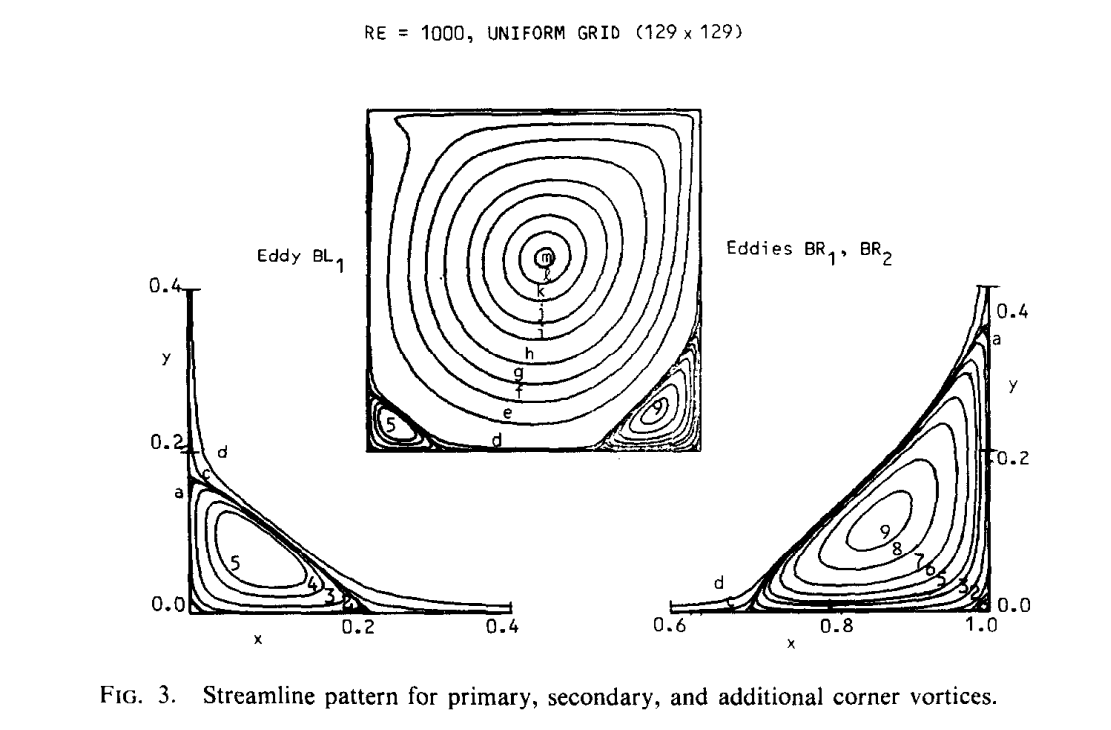
\includegraphics[width=.9\textwidth]{./img/ghia_solution_Re1000}
    \caption{Solution from Ghia et al. \cite{Ghia1982HighReSF} for the lid-driven cavity flow at $Re = 1000$.}
    \label{fig:ghia_solution_Re1000}
\end{figure}

After running the \acrshort{scgs} algorithm, we obtained the solution reported in Figure \ref{fig:scgs_solution_Re1000}.

\begin{figure}[H]
    \centering
    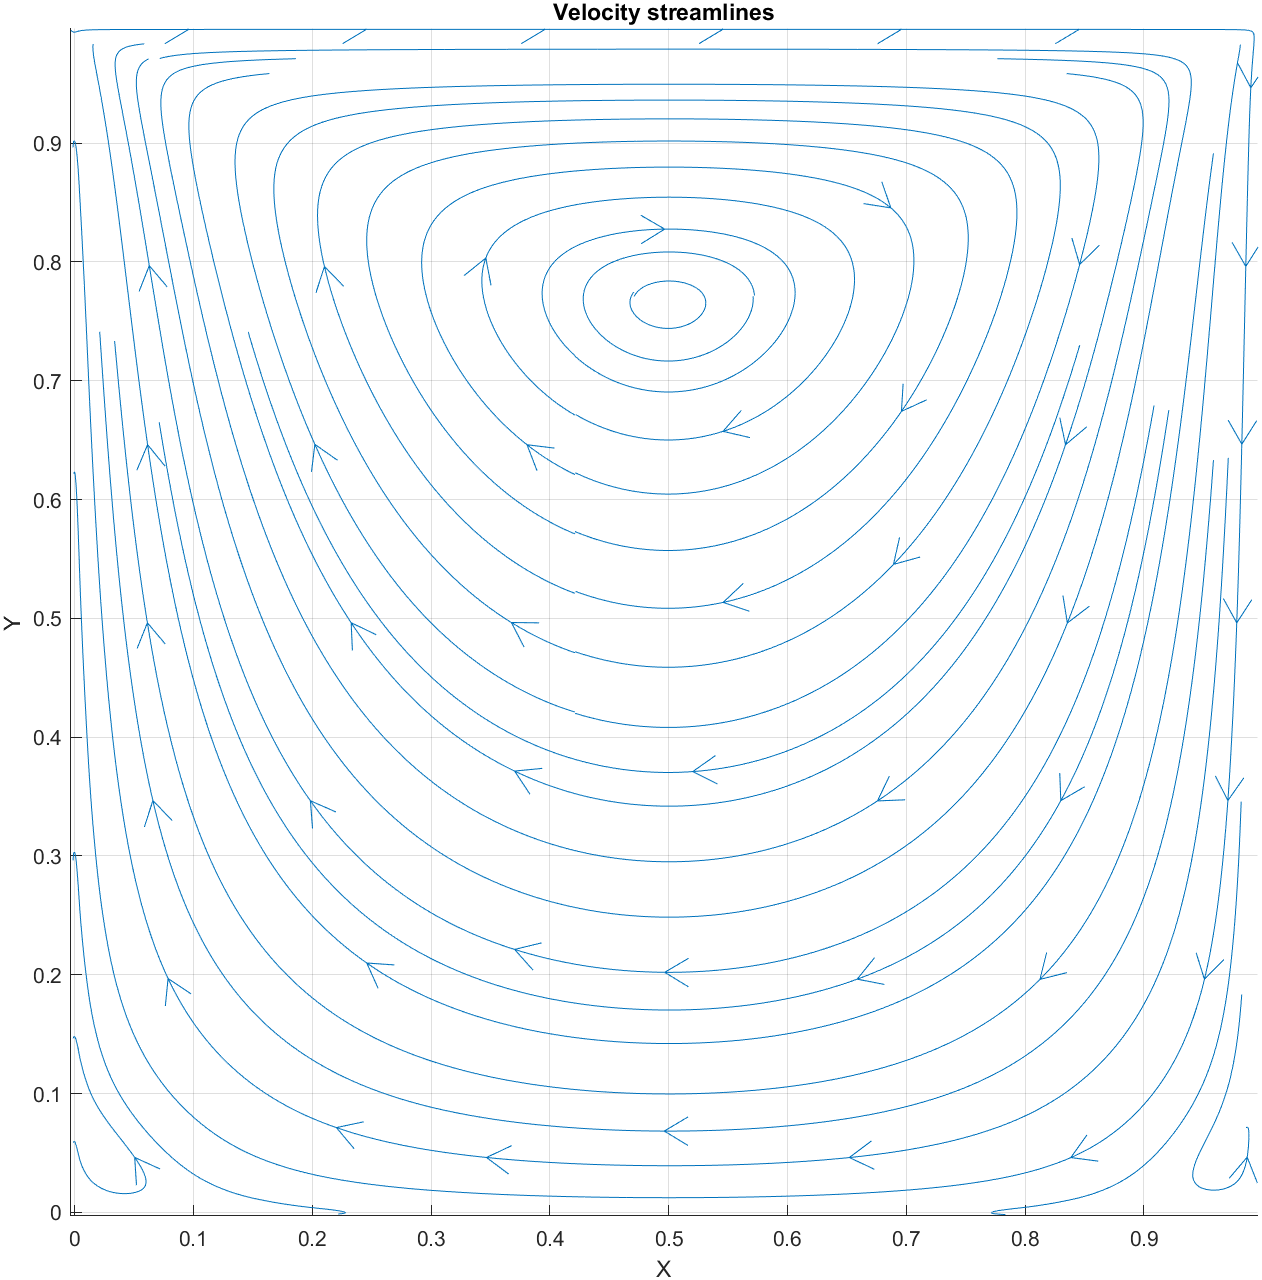
\includegraphics[width=.6\textwidth]{./img/scgs_solution_Re1000}
    \caption{Solution obtained using the \acrshort{scgs} algorithm for the lid-driven cavity flow at $Re = 1000$.}
    \label{fig:scgs_solution_Re1000}
\end{figure}

As it is easy to observe from the streamline plots, the solution obtained using our code is not in agreement with the one reported by Ghia.

In particular, the eddies at the bottom corners of the cavity are not present in our solution, and the overall distribution of the streamlines is basically symmetrical which intuitively is not correct.

Similar considerations can be made by comparing numerically the velocity profiles between the two solutions.

From Figure \ref{fig:velocity_profiles_Re1000_comparison} it's clearly visible how the two solutions are not in agreement.

\begin{figure}[H]
    \begin{minipage}[b]{0.45\textwidth}
        \centering
        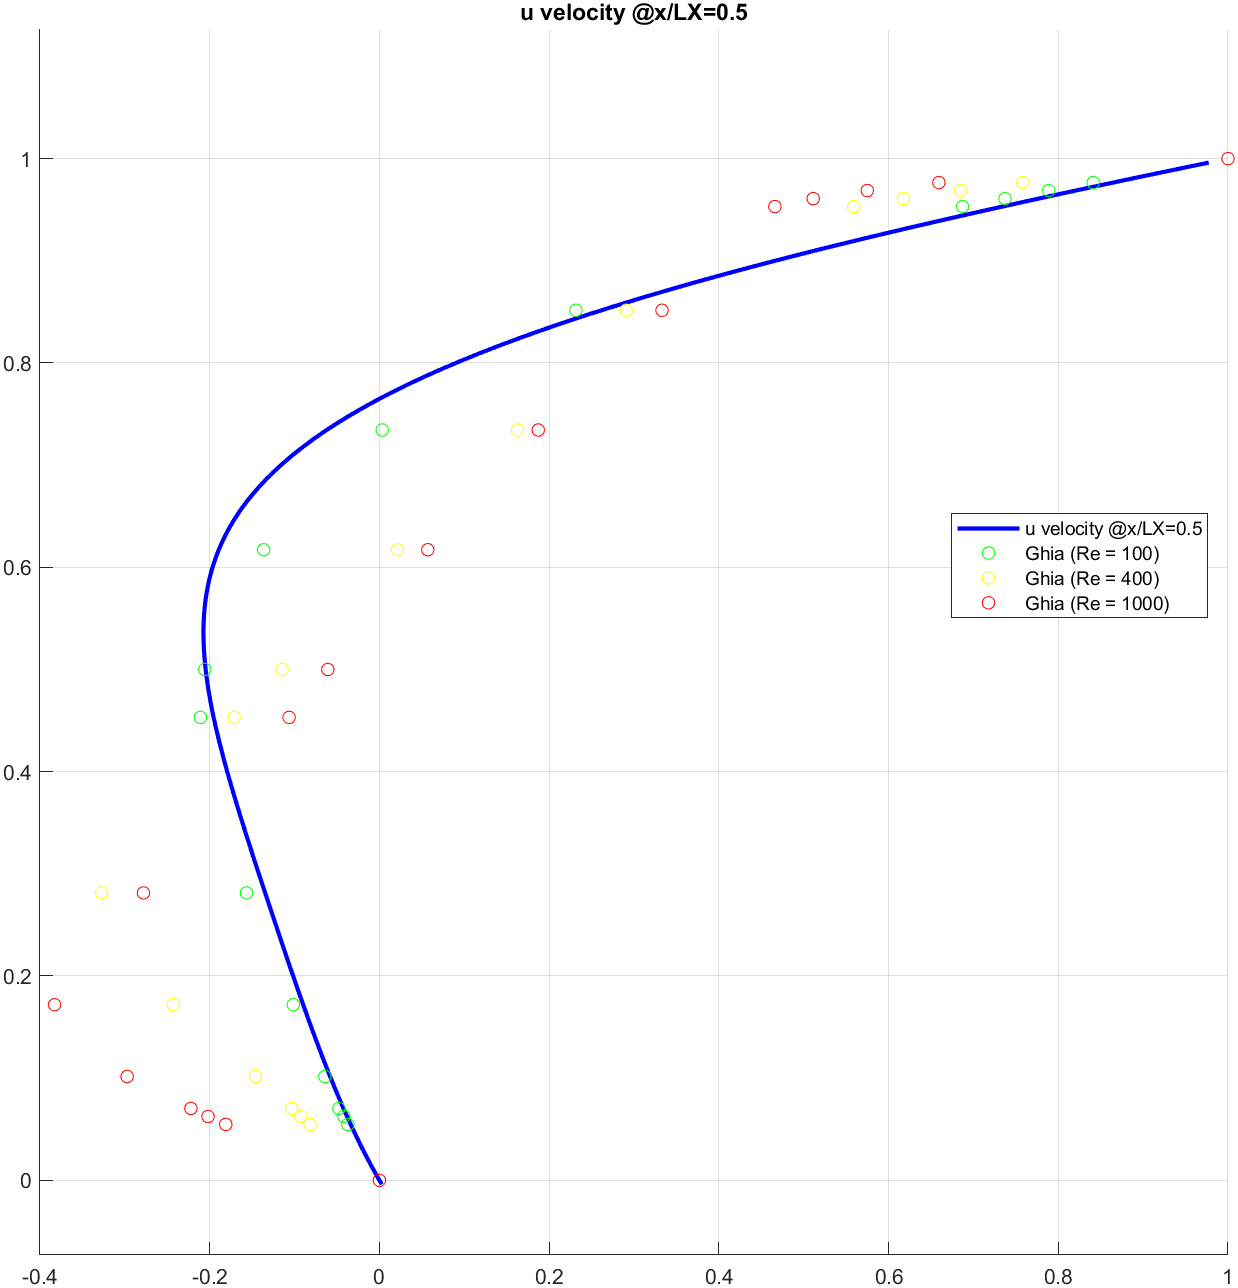
\includegraphics[width=.9\textwidth]{./img/velocity_profiles_Re1000_u}
        \caption{$u(y) @ x/L_x = 0.5$}
        \label{fig:velocity_profiles_Re1000_u}
    \end{minipage}
    \hfill
    \begin{minipage}[b]{0.45\textwidth}
        \centering
        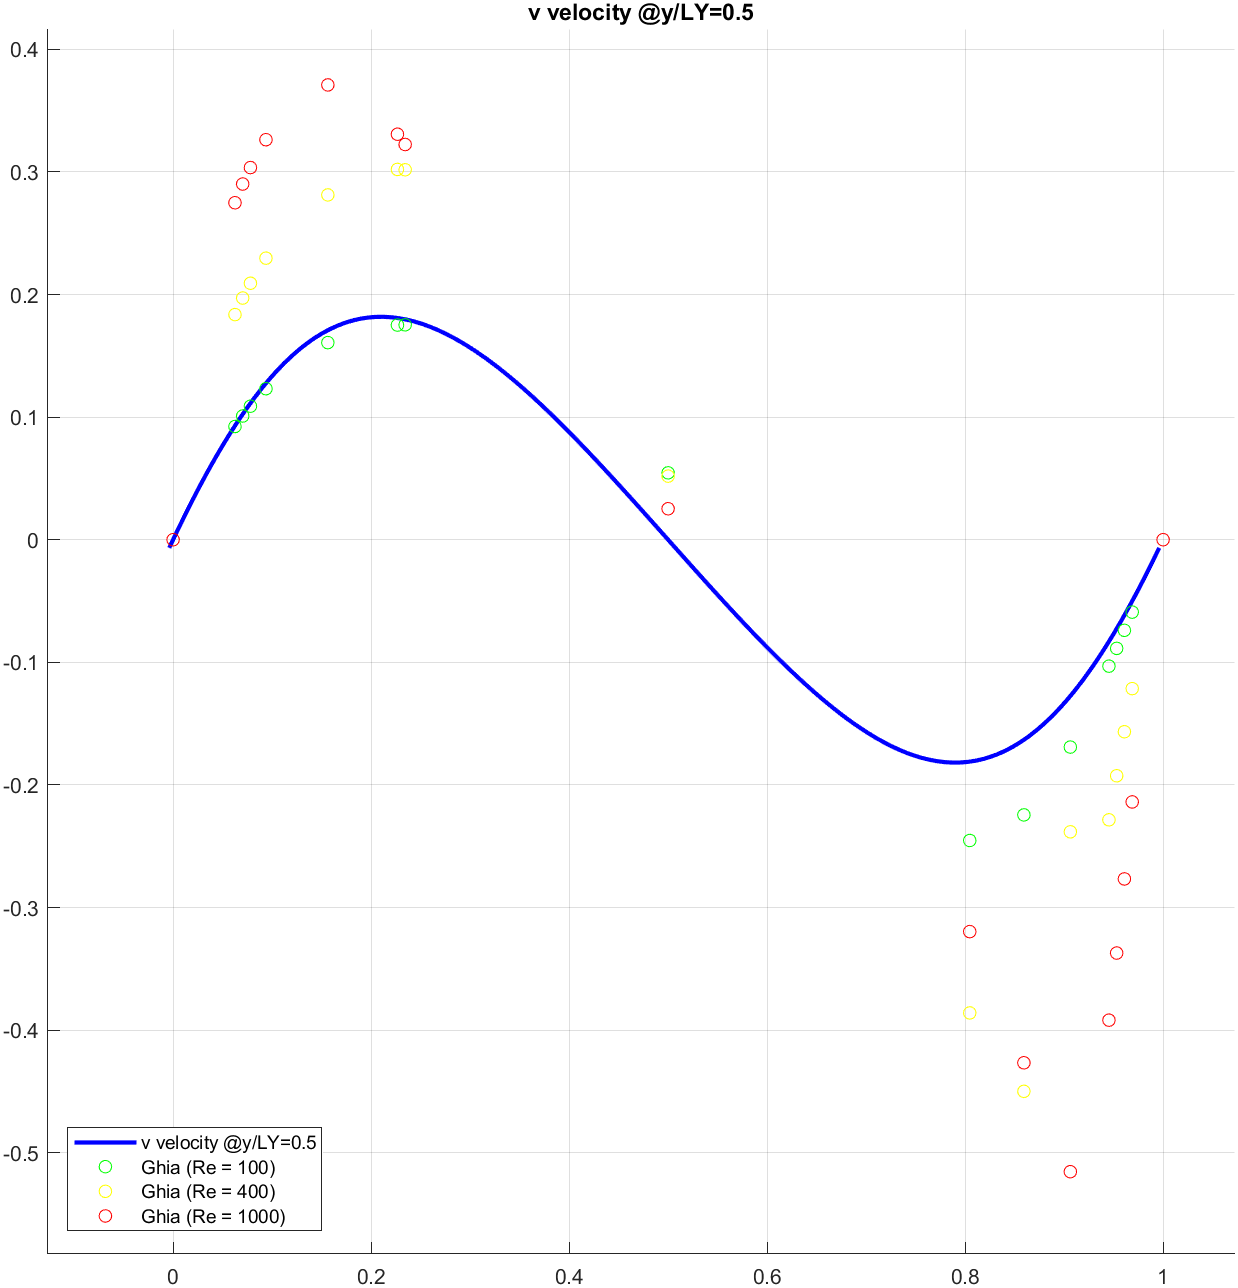
\includegraphics[width=.9\textwidth]{./img/velocity_profiles_Re1000_v}
        \caption{$v(x) @ y/L_y = 0.5$}
        \label{fig:velocity_profiles_Re1000_v}
    \end{minipage}
    \caption{Comparison of the velocity profiles.}
    \label{fig:velocity_profiles_Re1000_comparison}
\end{figure}

We also have tried to run the code with different parameters, but the results are always not in agreement with the ones reported by Ghia et al. \cite{Ghia1982HighReSF}.

\paragraph{Note}

We will try to fix the bug and update the results as soon as possible.
Not for the assegnment or the mark related to it, but for the sake of the project itself (it's useless to have a code that doesn't work as expected\dots).
